%!TEX root = ../NCVC3.tex

\mysection{CADでの作図}

\vspace*{1zh}
 旋盤データ生成における,基本的な作図方法を解説します.
既知部分は省略されていますので著書『いまからはじめるNC工作第2版』も併せて参照してください.

%\begin{figure}[H]
%\centering
%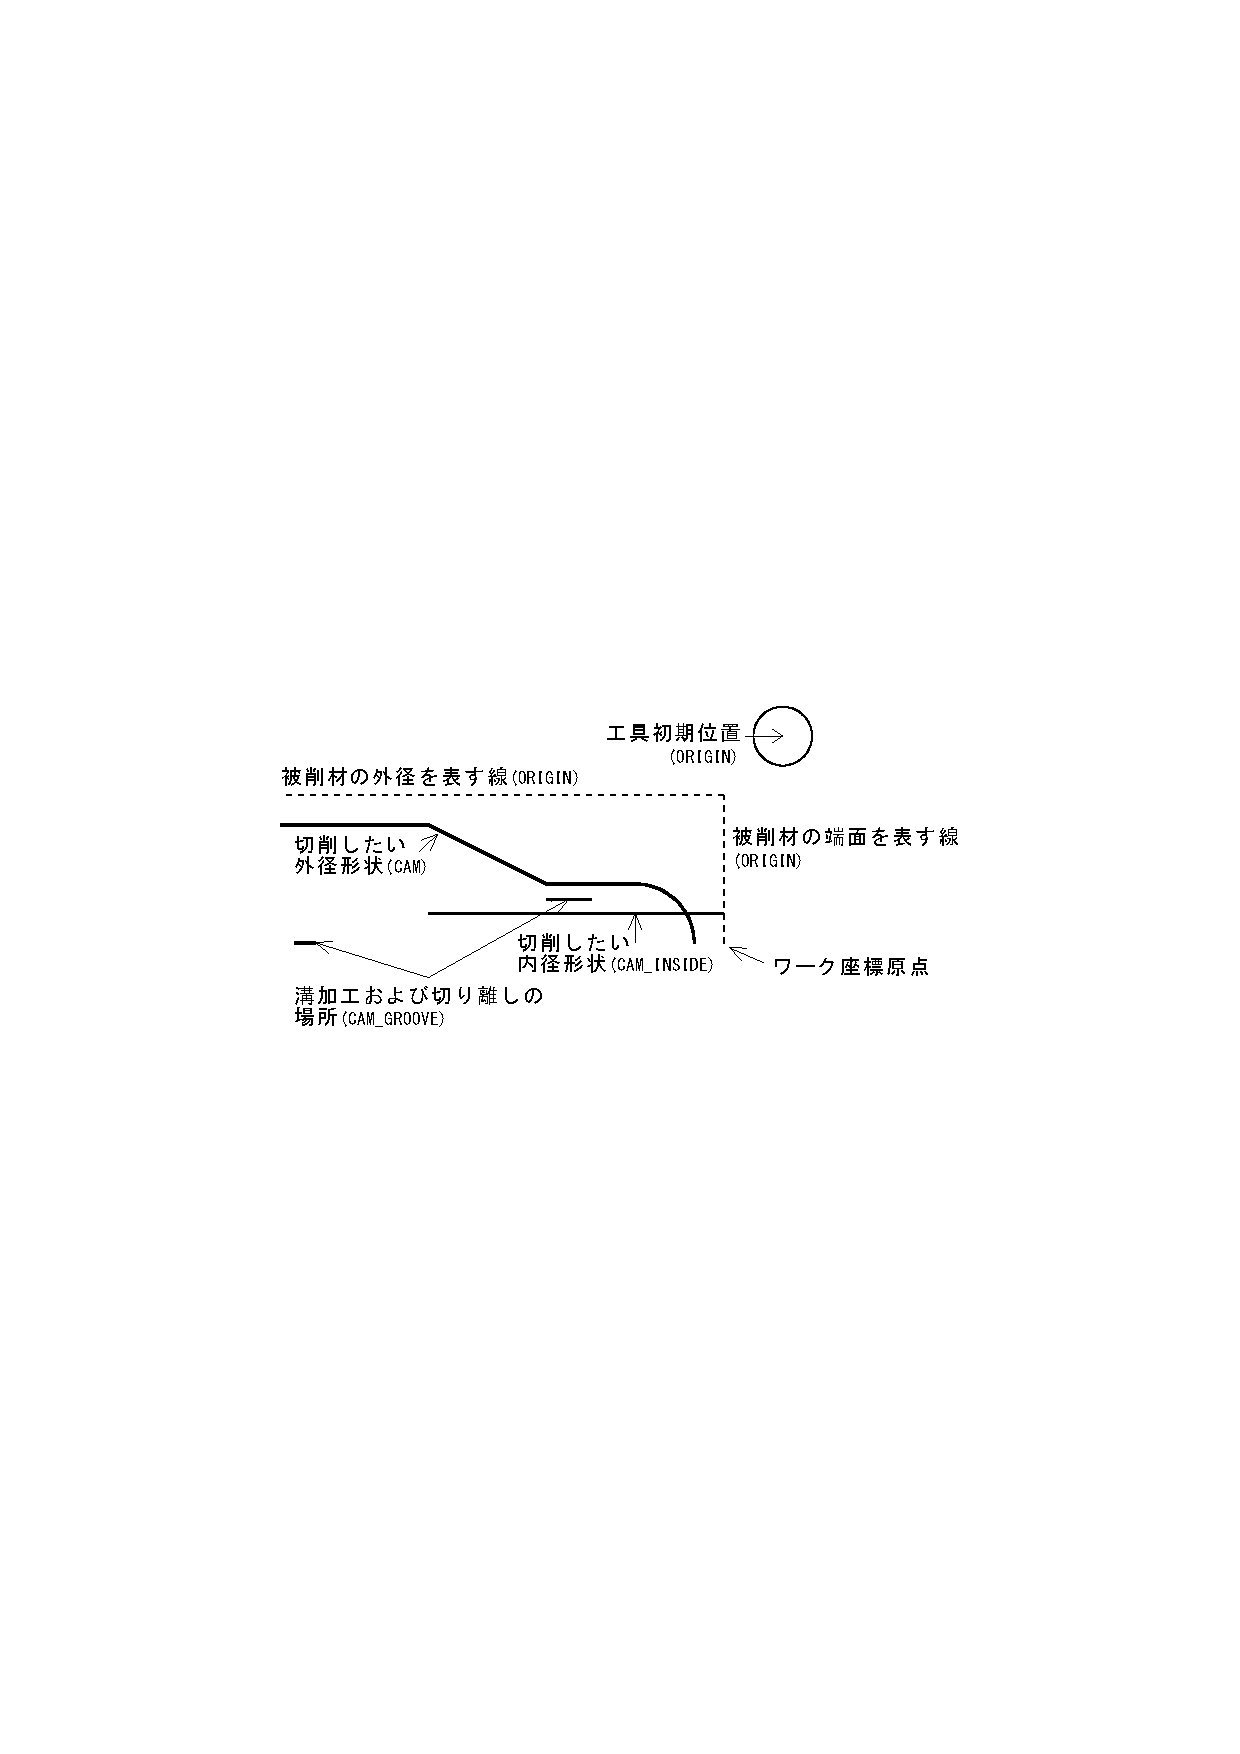
\includegraphics{No1/fig/sample.pdf}
%\caption{サンプル図形}
%\label{fig:sample.pdf}
%\end{figure}

 ORIGINレイヤの原点を示す円の中心が,ZX座標の工具初期位置となります.
さらに,被削材(丸棒)の端面と外径を表す直線を作図してください.
とくに端面を表す線の一番下の座標はワーク座標原点の意味もあり,ここがZ=0, X=0の認識で生成されます.

 CAMレイヤは,フライス加工と同様に切削形状を作図しますが,フライス加工では工具軌跡が基本なのに対し,旋盤加工では最終的に必要な形状を作図します.

 内径形状を示す作図は,外径形状とは別のレイヤに作図し,INSIDEという名前を追加してください.

 突っ切りバイトによる溝加工や切り落としは,GROOVEという名前を追加したレイヤに直線を作図してください.

 NCVCでの読み込みは従来通りです.
ORIGINレイヤに工具初期位置を示す円と2つの直線が読み込まれると,旋盤生成のメニューがアクティブになります.

%\begin{figure}[H]
%\centering
%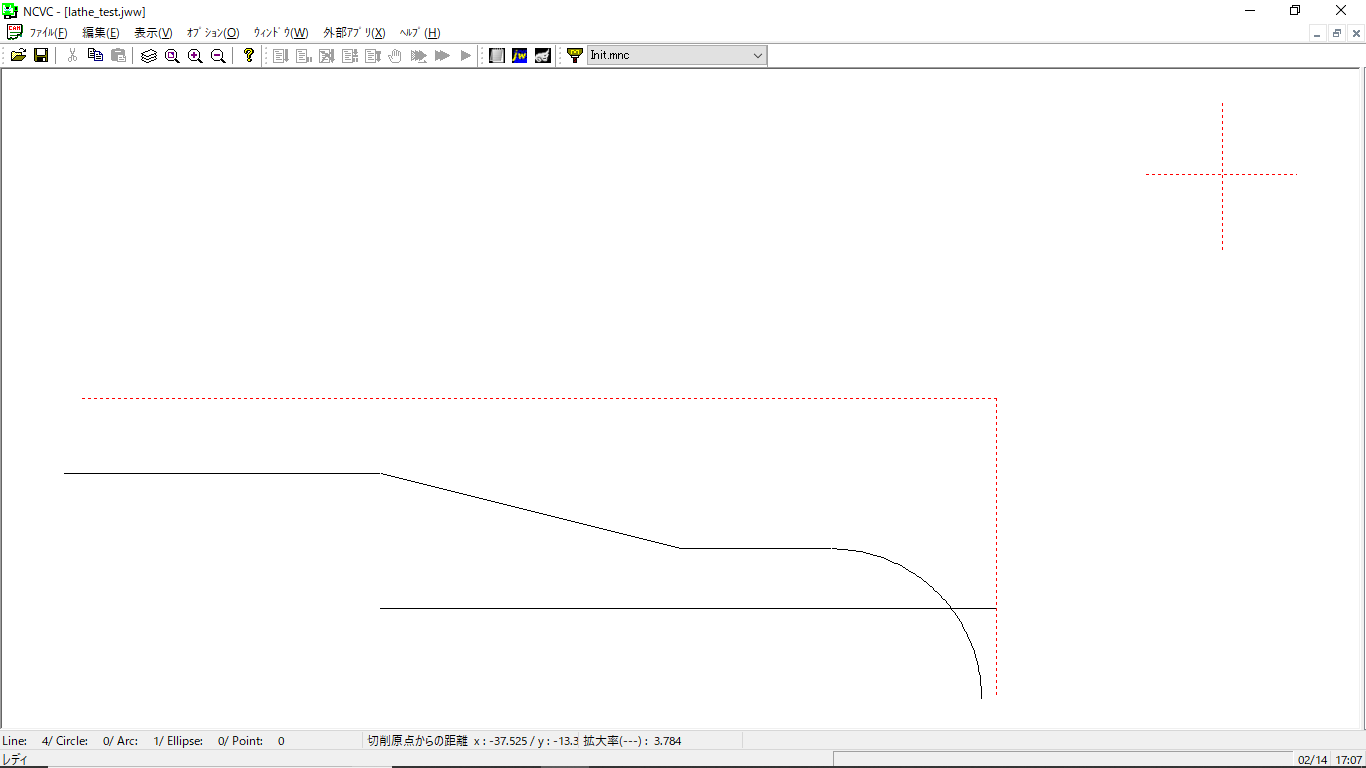
\includegraphics[scale=0.5]{No1/fig/read.png}
%\caption{CADデータの読み込み}
%\label{fig:read.png}
%\end{figure}
